\section{Unblinding results}

This search for a new dark boson is done blindly to ensure that no bias is introduced in the
course of the analysis.
The data is unblinded in stages to ensure that the selection is behaving as expected on real data.

Before any unblinding, the selection is checked using selected candidates
consistent with the decay \decay{\Bd}{\jpsi\Kstarz}.
The selection applied in the \sm analysis of \btokstrmumu, as described in
\Ref{LHCb-CONF-2015-002}, yields $320\,000$ candidate decays.
Using the selection from \Sect{sec:db:sel} and approximately \approx$260\,000$
\decay{\Bd}{\jpsi\Kstarz} candidates remain.
Therefore only \approx$10\%$ fewer events in this selection, which is not surprising
considering this search is for a much rarer process than \decay{\Bd}{\Kstarz\mumu} in the \sm, and
therefore selection requirements are likely to be tighter.

Selected \decay{\Bd}{\jpsi\Kstarz} events are also used to check that the selection was not biased
based on neither the year, nor the polarity of the \lhcb magnet.
No bias is observed, in fact
efficiencies for the \uBDT are observed to be consistent to the $10^{-4}$ level in all four regions.

The unblinding procedure begins by checking the yield of the normalization channel
\btokstrmumu in the range $1.1<\qsq<6.0\gevgev$ and comparing it with the yield from the \sm
analysis.
The yield is taken from an unbinned fit to selected prompt \btokstrdb candidates using a mass model
of two Gaussian functions sharing the same mean, and with a power-law tail on the low mass side.
%same fit model for the signal component as used in \Ref{LHCb-CONF-2015-002}, which is the sum of
A simple exponential models the background component.
This yields 527 \Bd candidates, which can be compared to \approx$625$ events in the \sm selection,
where the drop in signal is, again, expected given the search is for a rare process.
Together with the drop in signal, comes a drop in background yield, from \approx$630$ background
events over the full mass range, to only 290.
Figure~\ref{fig:db:norm} shows the \Bd candidate mass spectrum for the normalization channel, and
the fitted distribution overlayed.

\begin{figure}
  \begin{center}
    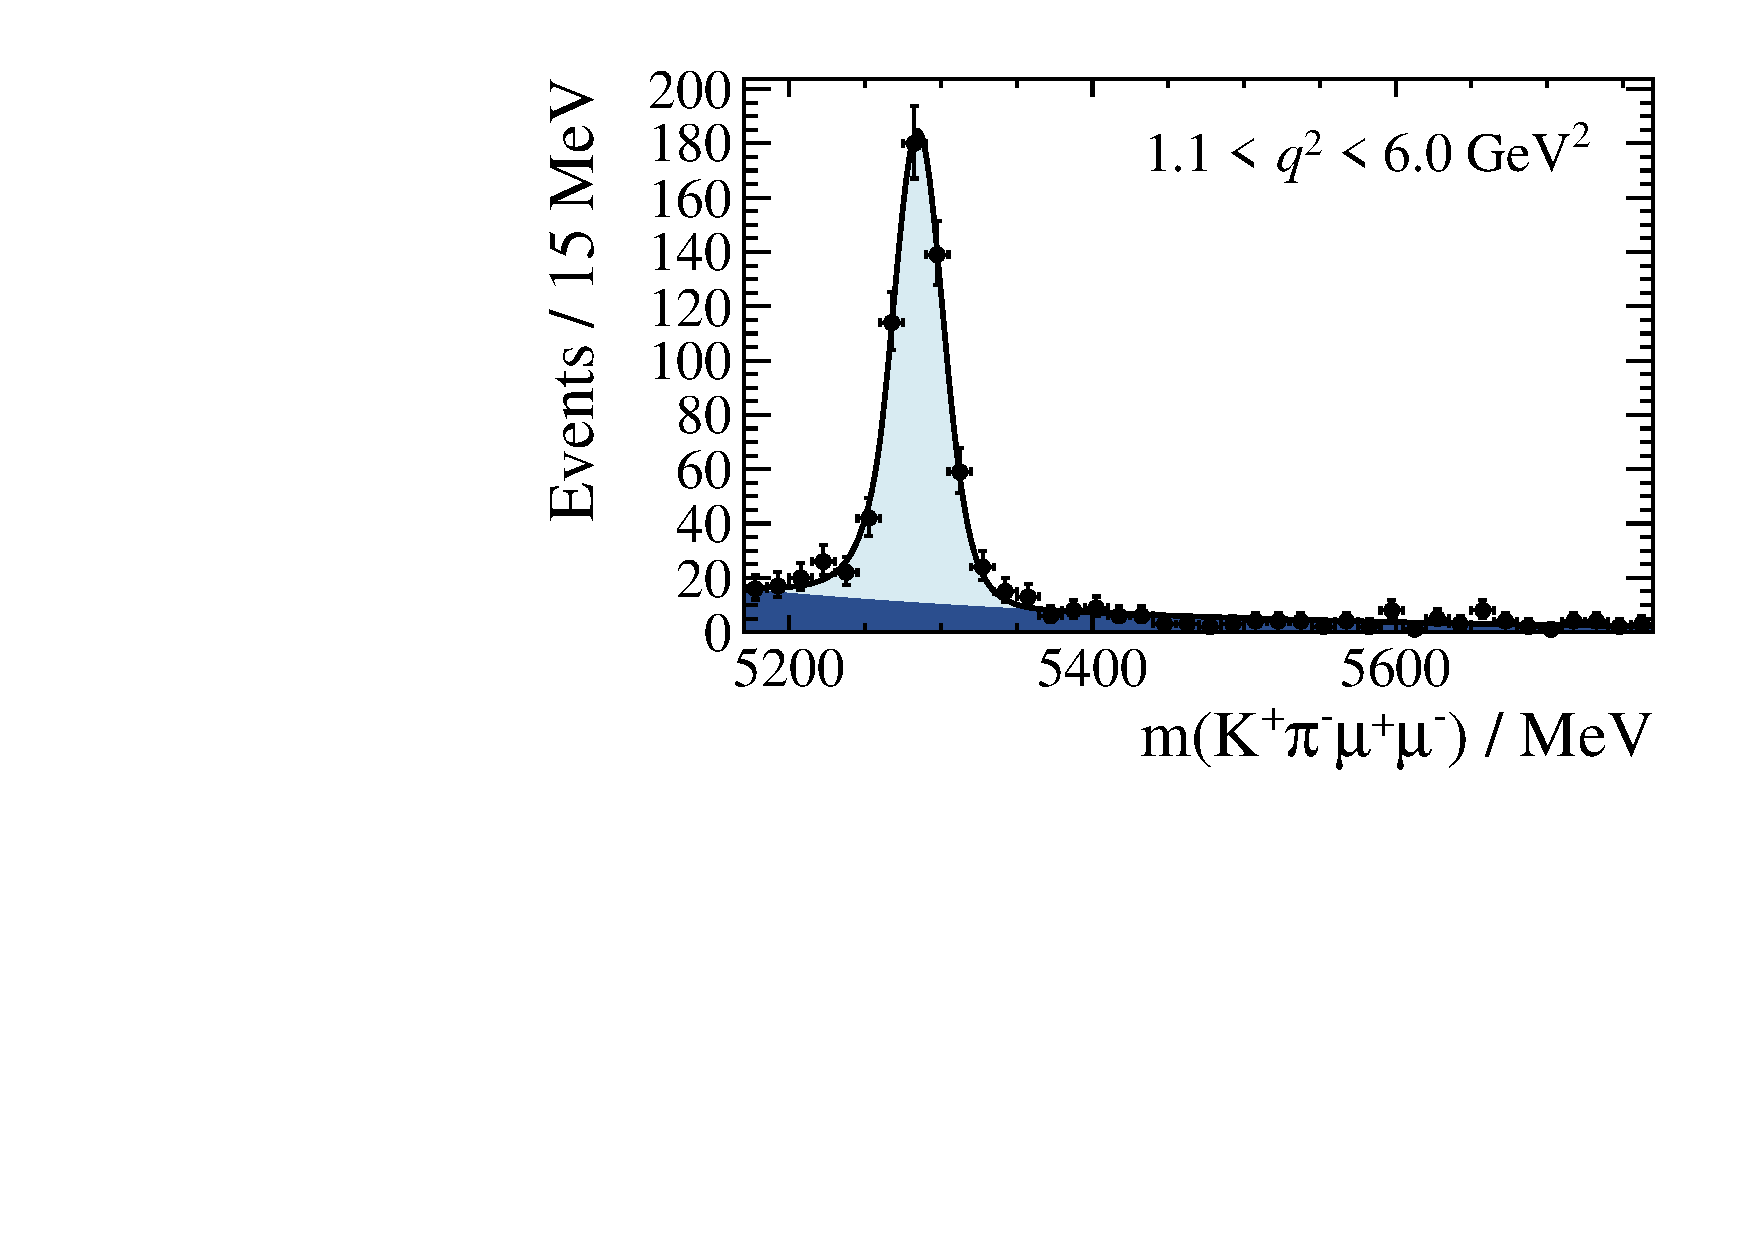
\includegraphics[width=0.48\textwidth]{norm_channel}
    \caption[Fit to the normalization channel, \btokstrmumu in the range $1.1<\qsq<6.0\gevgev$]
    {
      Fit to the invariant mass spectrum of the \Bd candidates in selected data in the range
      $1.1<\qsq<6.0\gevgev$.
      The signal model is the sum of two Gaussian functions with power-law tails on the low-mass
      side with parameters taken from the analysis described in
      Ref.~\protect\cite{LHCb-CONF-2015-002},the background model is a decaying exponential.
      This fit results in a signal yield of $(527\pm26)$ compared to approximately 625 in the \sm
      analysis.
      %for more in depth numbers, please refer to Table~\protect\ref{tab:db:nums126}.
    }
    \label{fig:db:norm}
  \end{center}
\end{figure}

After unblinding the region $1.1<\qsq<6.0\gevgev$, other prompt \qsq regions were also used to
confirm that the ratio of \bdt selection efficiencies
$\varepsilon_\mathrm{BDT}^\mathrm{\qsq bin}(\btokstrmumu) / \varepsilon_\mathrm{BDT}(\btojpsikstr)$
are approximately the same in data and simulation.
To determine these efficiencies, the full selection without the \BDT is taken, and a fit performed
and the signal yield is extracted.
Next, the \BDT is applied and a second fit is performed, then take the ratio of the signal
yields.
A comparison between these numbers in data and simulation is shown in comparison is shown in
\Fig{fig:bdtEffRatio}, the two distributions are shown to be in good agreement, centred around
unity with about 5--10\pc precision.
%This approach ignores the fact that there may be some small peaking background component that gets
%counted as signal pre-BDT cut, but is removed by the BDT.
%Note, however, that in the
%$\varepsilon_\mathrm{BDT}^\mathrm{\qsq bin} / \varepsilon_\mathrm{BDT}^{\decay{\Bd}{\jpsi\Kstarz}}$
%ratio, only the difference in peaking background contributions matters.
%Given that all peaking backgrounds that are visible in the various 2-body mass combinations are
%explicitly vetoed, no peaking background contributions at the level of the statistical precision of
%this test are expected.

\begin{figure}
  \begin{center}
    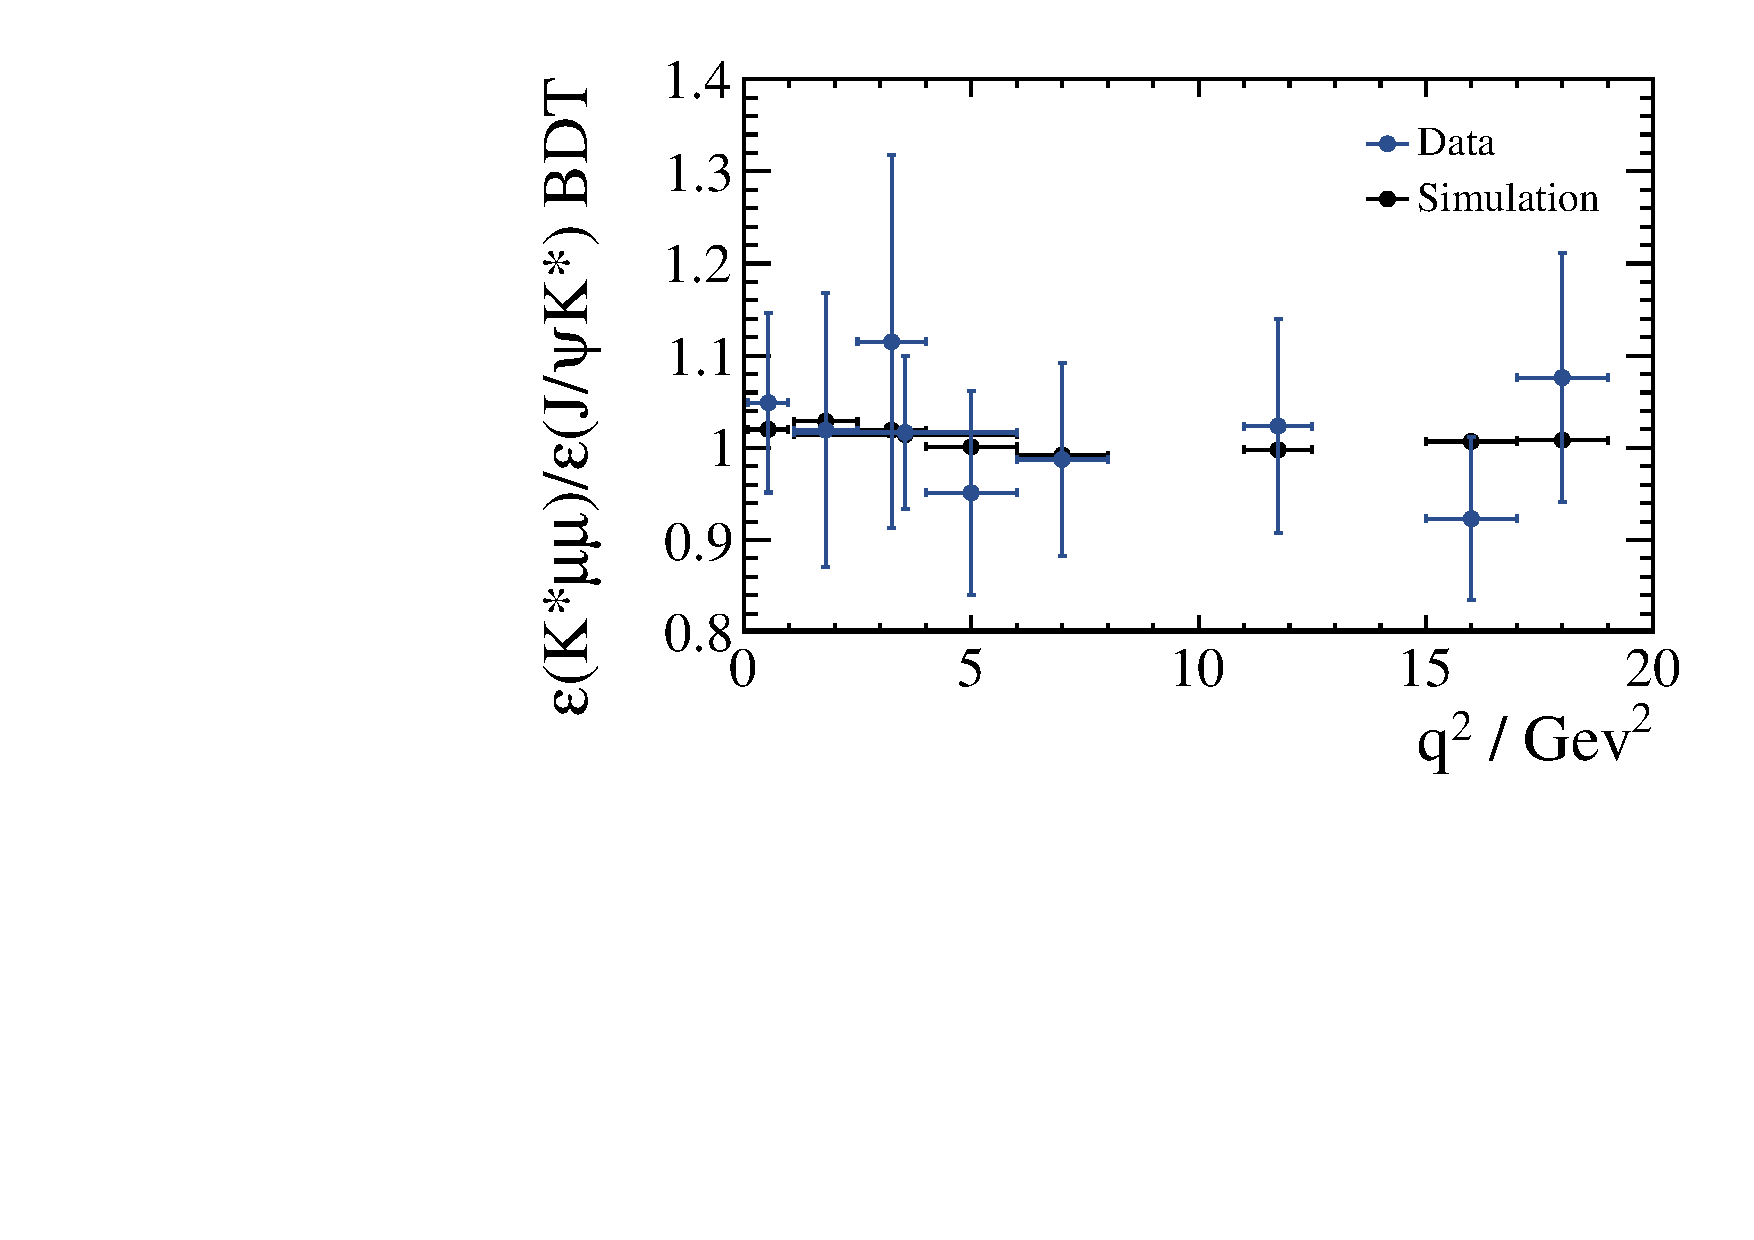
\includegraphics[width=0.48\textwidth]{bdtEffRatio}
    \caption{
      Ratio of the efficiencies of the \bdt selection for a range of \qsq bins, as used in the SM
      \btokstrmumu analysis, with respect to the efficiency for \decay{\Bd}{\jpsi\Kstarz}.
      Data and simulation are shown to be in good agreement.
    }
    \label{fig:bdtEffRatio}
  \end{center}
\end{figure}

Using the unblinded distributions it is possible to estimate the amount of combinatorial background
that will remain in the final selection.
Fitting an exponential to model the background across the signal region allows an approximate
number of events in the combinatorial background to be deduced.
This number of events can be taken from the upper-mass sideband, and the invariant mass of the
dimuon pair can be plotted.
With this method, it expected that a maximum of 10(2) events will contribute to the background in
the prompt(displaced) region at a single test mass, but on average the value is 1.8(0.2) events per
bin.
Figure~\ref{fig:db:comb} shows the shape and scale of the combinatorial background, and the fits
used to calculate it.

\begin{figure}
  \begin{center}
    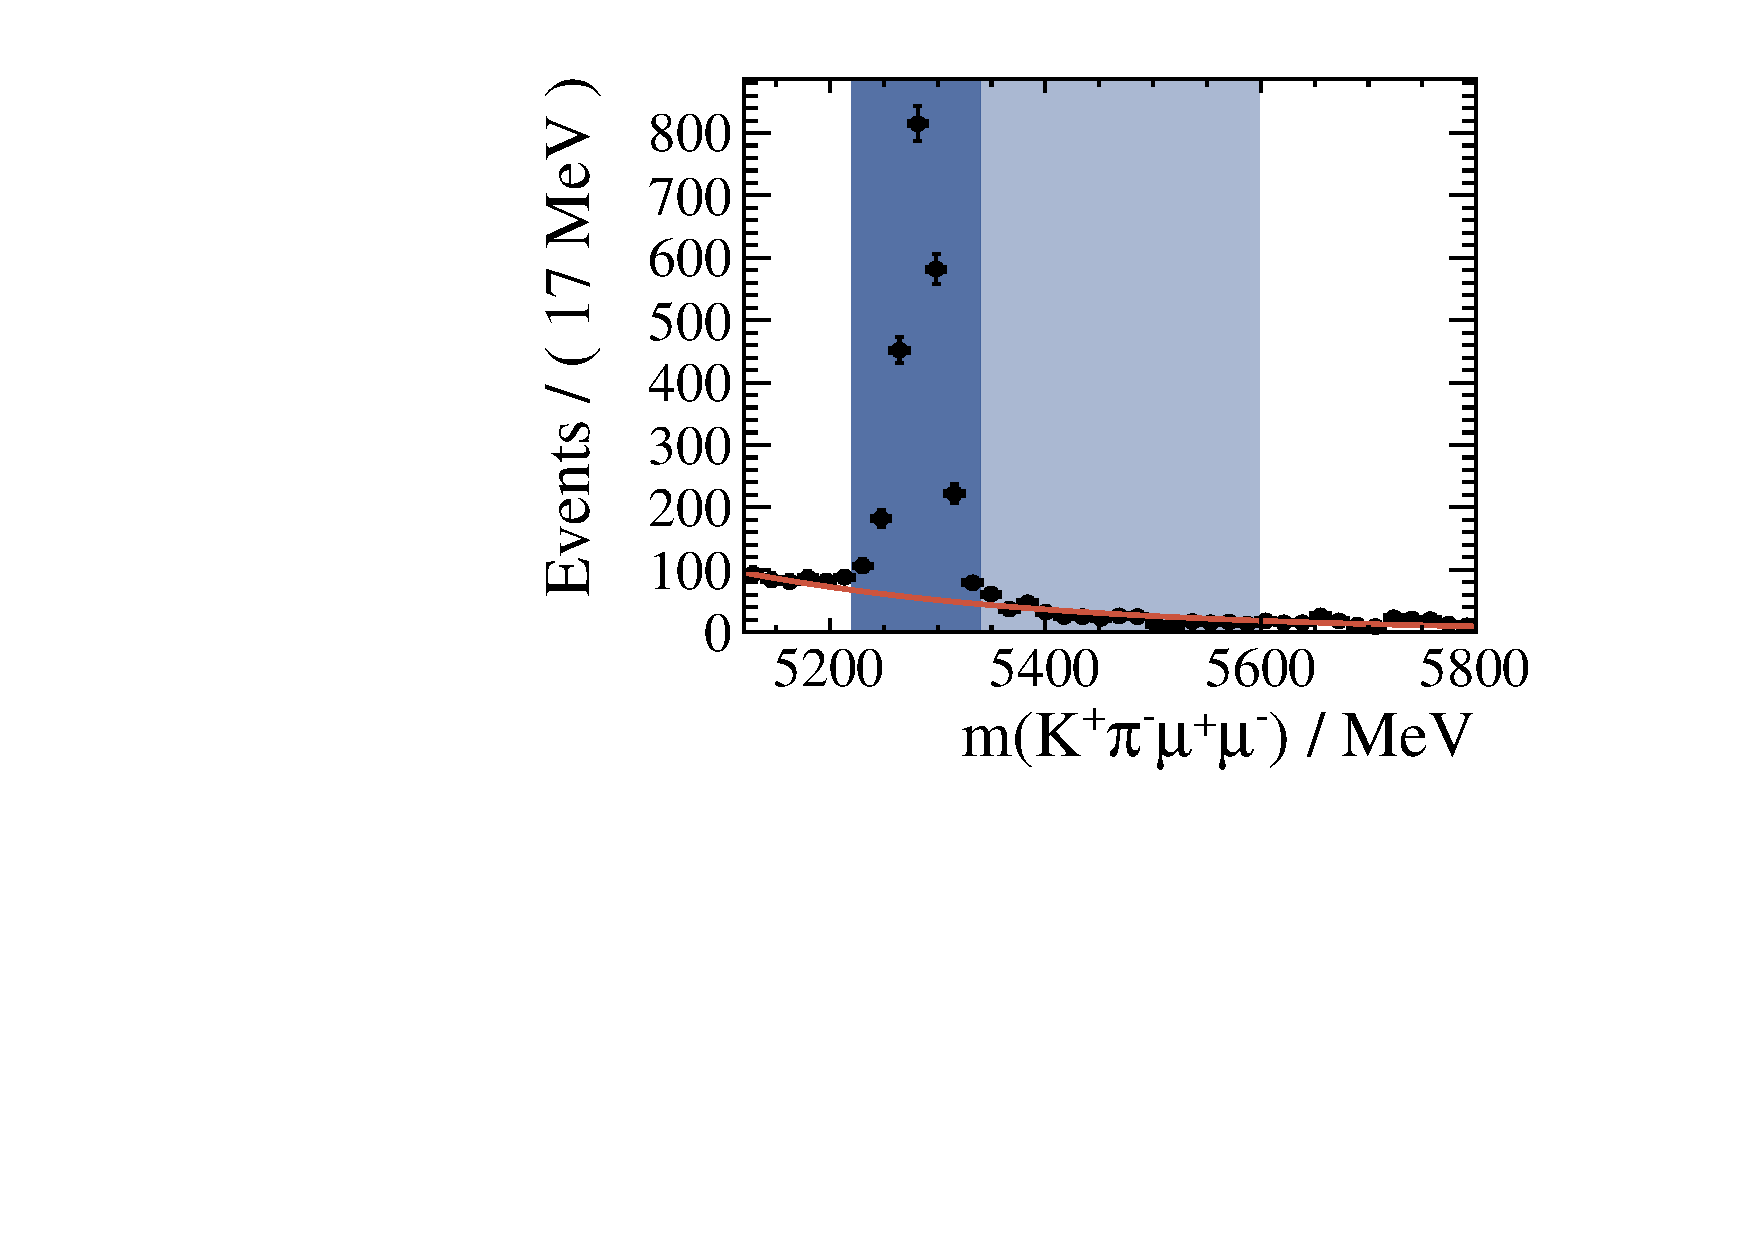
\includegraphics[width=0.48\textwidth]{combinatorial_prompt_fit}
    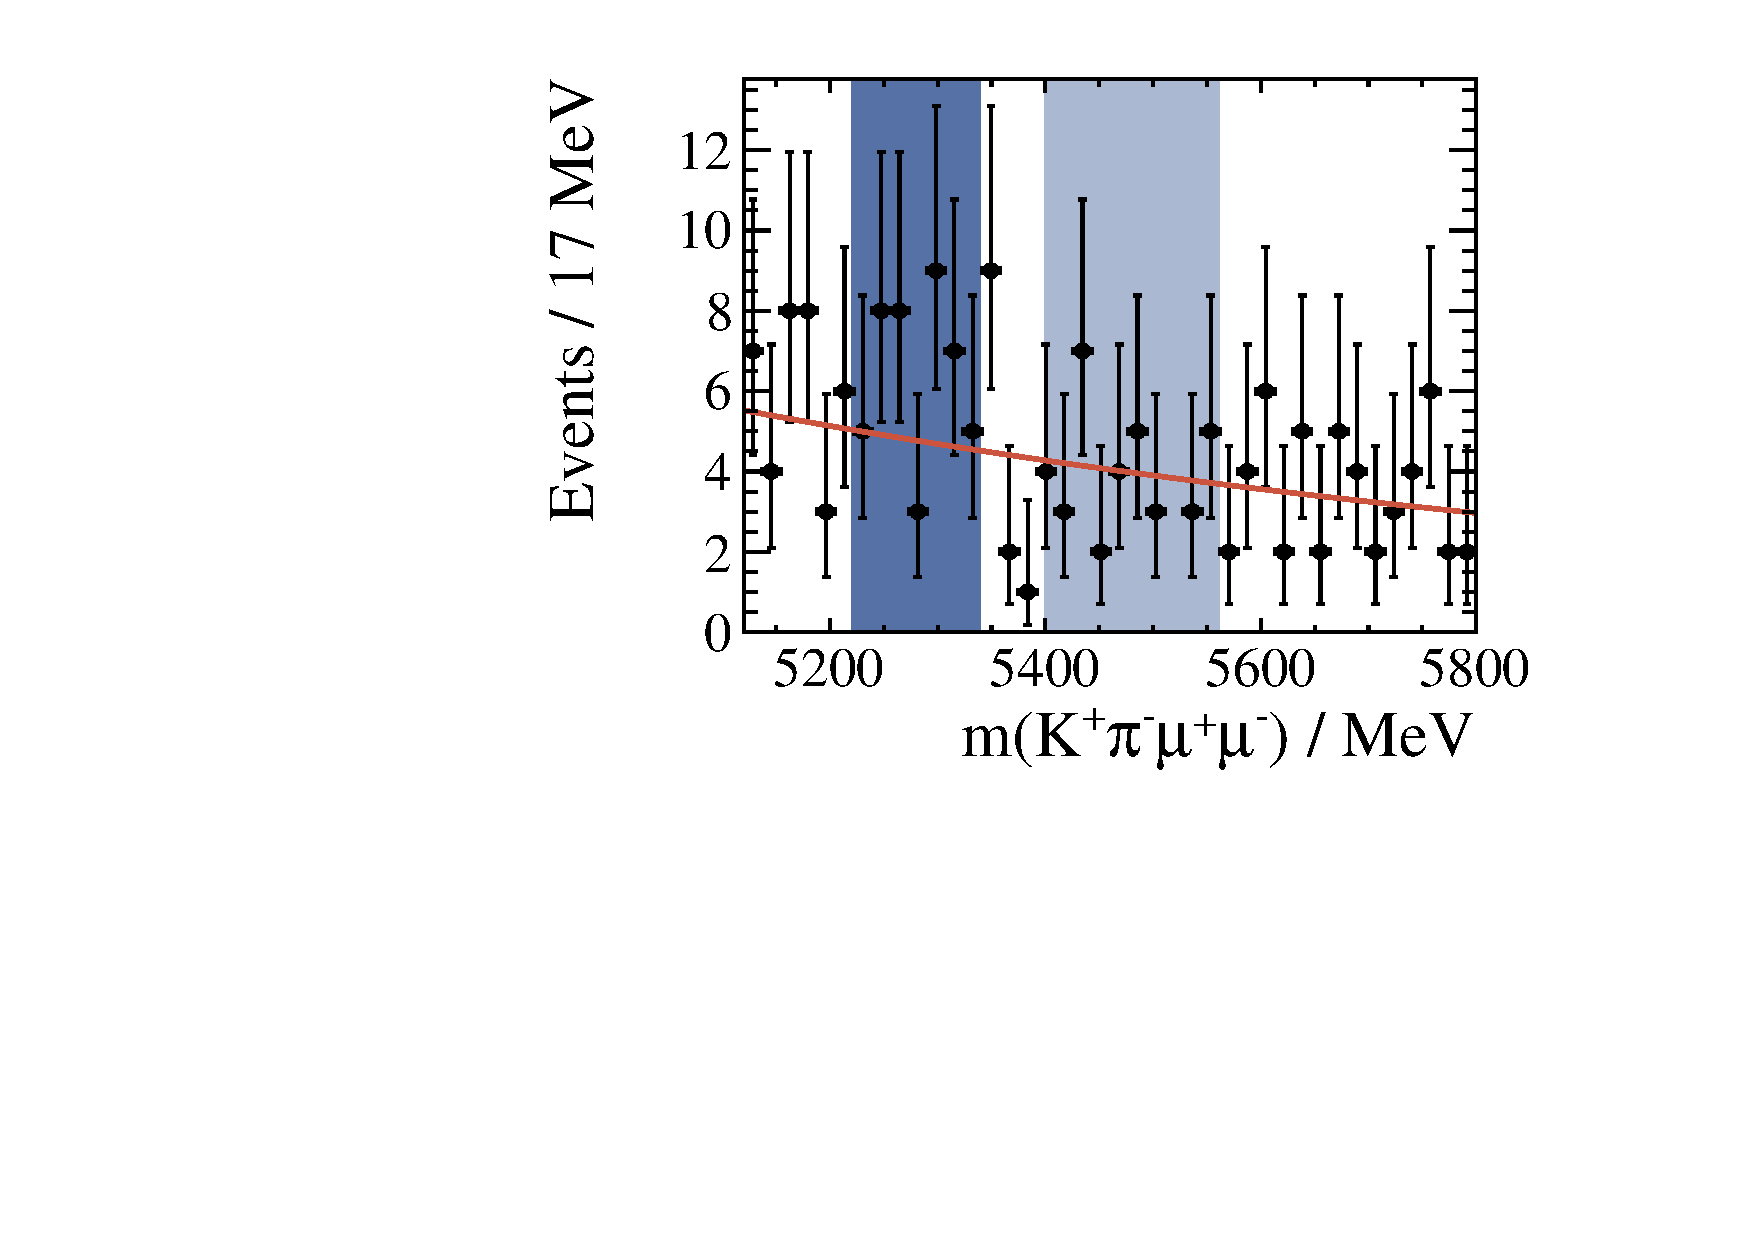
\includegraphics[width=0.48\textwidth]{combinatorial_displaced_fit}
    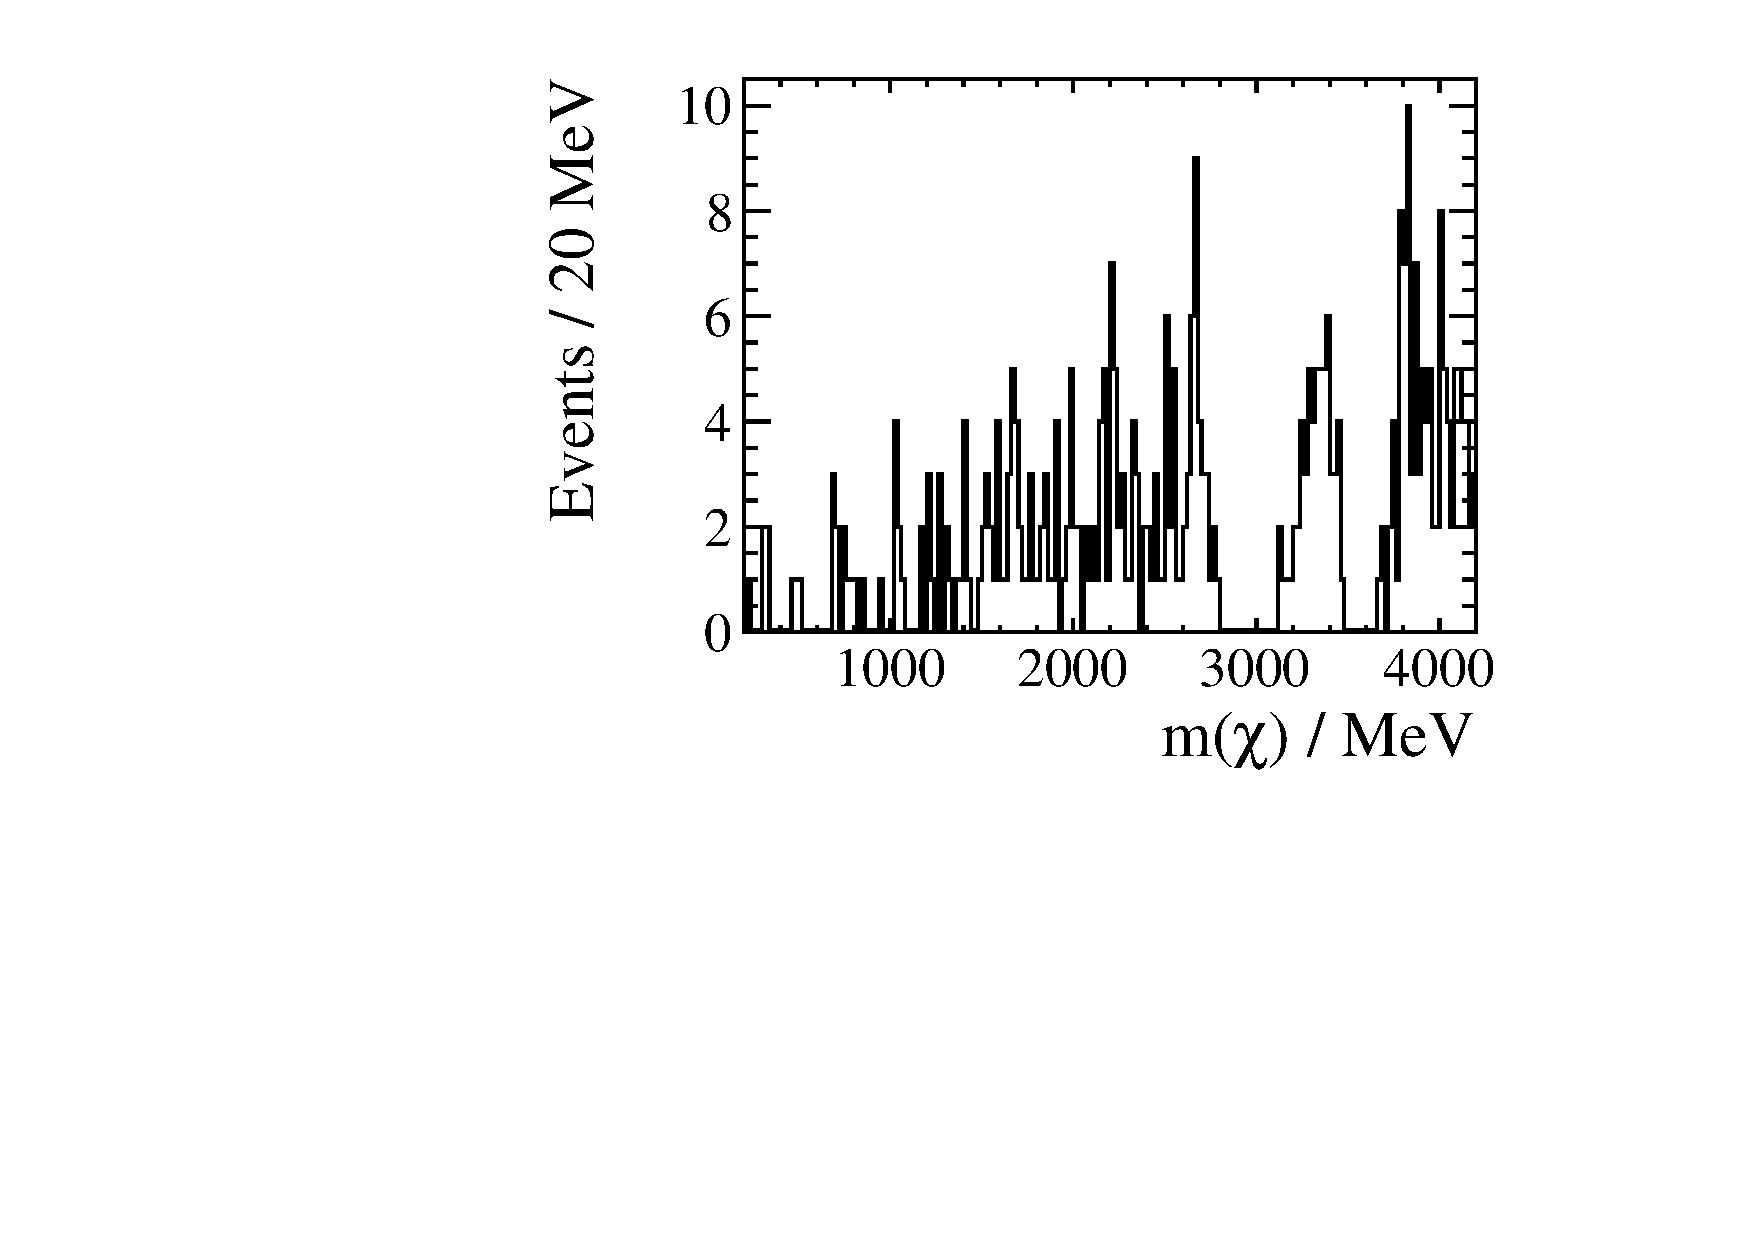
\includegraphics[width=0.48\textwidth]{combinatorial_prompt}
    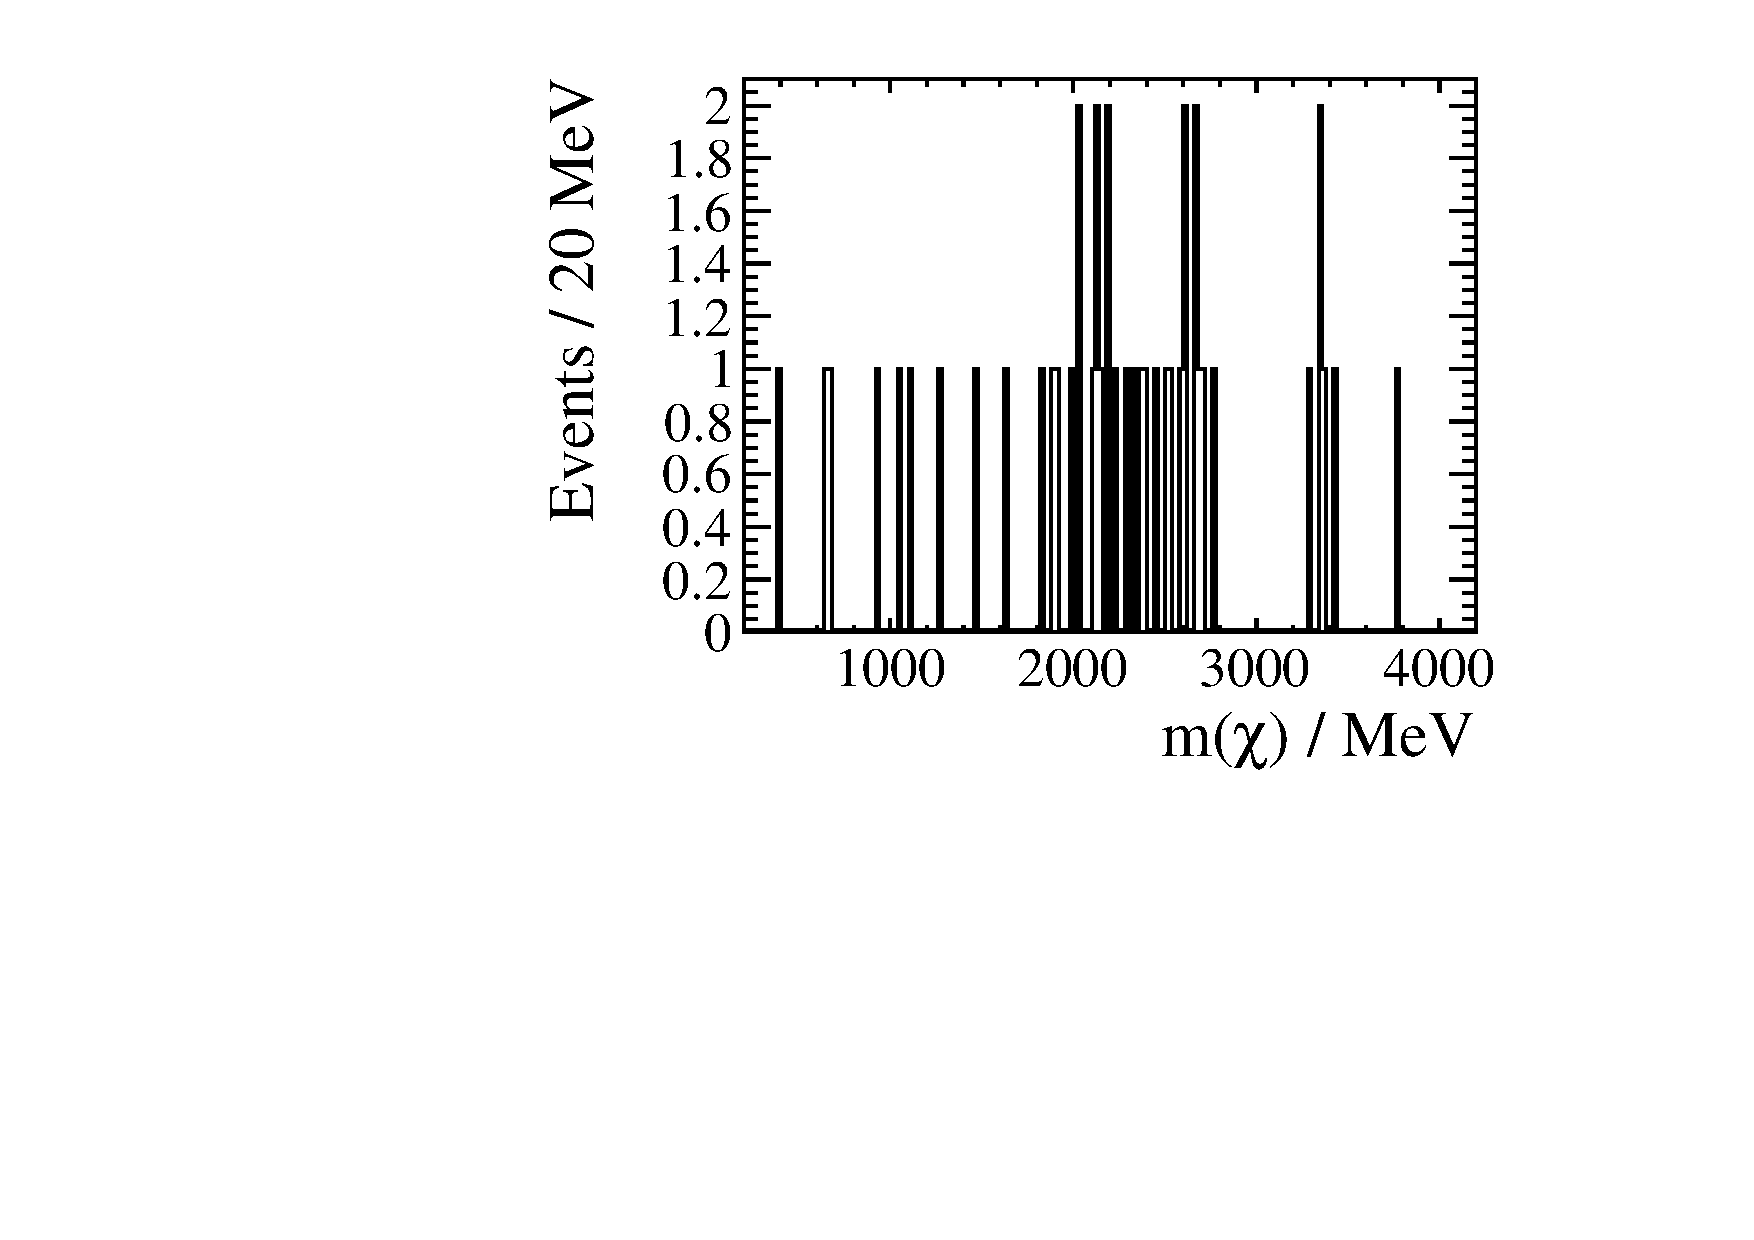
\includegraphics[width=0.48\textwidth]{combinatorial_displaced}
    \caption[Estimation of combinatorial background contribution]
    {
      Fits to the background component of selected \btokstrmumu events are shown in the upper
      plots, where the dark blue regions are not used in the fit, but are used to determine the
      number of events contributing to the combinatorial background by integrating across the
      region.
      The light blue region is covers the same number of background events as in the darker region,
      these are purely combinatorial background, and the invariant dimuon masses are plotted below,
      using a bin width that is approximately equal to the signal region in where the resolution is
      at its worst.
    }
    \label{fig:db:comb}
  \end{center}
\end{figure}



%At the time of writing, the unblinding procedure is no further than indicated above.
%As time progresses the whole dataset will be unblinded.
%First in binned distributions
%--- which will hide any potential signal, assuming the signal is not extremely obvious ---
%in the prompt and displaced regions.
%From these distributions toy datasets can be generated and used to convert the local minimum
%$p$-value to a global one, the procedure for which is described in \Sect{sec:db:strategy}.
%Systematic uncertainties will be evaluated and upper limits will be set for a range of \mass{\db}
%and \lifetime{\db}.

\subsection[Calculation of $p$-value]
{Calculation of $\boldsymbol{p}$-value}

The unblinded distribution in $m_{\mumu}$ is shown in \Fig{fig:db:mumu}.
Using the statistical method described in \Sect{sec:db:strategy} the following ranges in \mass{t}
are scanned:
\begin{align*}
  253.4 &< \mass{t} < \pz369.5 \mev \\
  574.5 &< \mass{t} < \pz906.5 \mev \\
  1136.0 &< \mass{t} < 2813.0 \mev \\
  3246.5 &< \mass{t} < 3576.5 \mev \\
  \intertext{and}
  3796.0 &< \mass{t} < 4356.0 \mev.
\end{align*}
Values of \mass{t} do not reach threshold boundaries because of the widths of the sidebands.
The minimum local $p$-value is found to be $3.6\e{-3}$ at $m_{t}^\mathrm{min} = 4285.0\mev$.

To convert the $p$-value to a global one, a \PDF is fit to the \mass{\mumu} distribution of the
prompt and displaced \btokstrdb candidates that lie outside of the vetoed regions, and outside of
the signal region centred at $m_t^\mathrm{min}$.
A fourth(second) order Chebychev polynomial is fit to candidates in the prompt(displaced) region.
From these \glspl{PDF} $1.5\e{7}$ toy datasets are generated, and the minimum $p$-value for each
one is calculated.
Constructing a cumulative distribution of these $p$-values makes an easy conversion from loval to
global $p$-values, this conversion is shown in \Fig{fig:db:mumu}.
Shown alongside the cumulative histogram is the asymptotic approximation, which is seen to be in
excellent agreement for local $p$-values less than about $10^{-4}$.
The histogram converts the local $p$-value to a global $p$-value of $0.63$, equivalent to a shift
in significance of $2.9\stdev$ to $0.48\stdev$.
These results show no evidence for a new dark boson in the mass ranges given above.

%253.4 -> 369.5
%574.5 -> 906.5
%1136 -> 2813
%3246.5 -> 3576.5
%3796 -> 4356
%3.610859e-03,  4285.035MeV => 2.9sigma
%0.63322 => 0.48sigma global
% RooStats::PValueTOSignificance(pval / 2)

%Firstly, the look-elsewhere effect must be accounted for, which
%is done using the method outlined in \Sec{sec:db:pval} using all dimuon pairs from \Bd candidates
%that fall within $2.5\stdev$ of the nominal \Bd mass.
%It was decided that if the global $p$-value corresponds to a evidence for a new particle
%($3\sigma$ or above) then fits will be used to
%determine the best-fit mass and lifetime of the excess.

%Figure~\ref{fig:db:mmumu} shows the unblinded dimuon mass distribution for the prompt and
%displaced regions, fitted to fourth order Chebychev polynomials.
%The displaced region is compatible with the expected contribution from combinatorial background.
%A toy dataset is generated using this \PDF, full statistical method is applied to find the
%$p$-value at each value of \mass{t}, and thus the minimum $p$-value for a single toy dataset is
%extracted.
%This process is repeated $10^7$ times, as required to achieve $p$-values corresponding to a
%significance of $5\stdev$.
%From the minimum $p$-values the fraction of toy datasets with minimum $p$-values less than some
%value can be computed, and thus a conversion from local to global minimum $p$-value for any given
%toy; therefore for the data itself.
%Figure~\ref{fig:db:mmumu} also shows this cumulative distribution of minimum local $p$-values from
%$1.5\e{7}$ datasets along with the asymptotic expectation~\cite{Gross:2010qma}.

\begin{figure}
  \begin{center}
    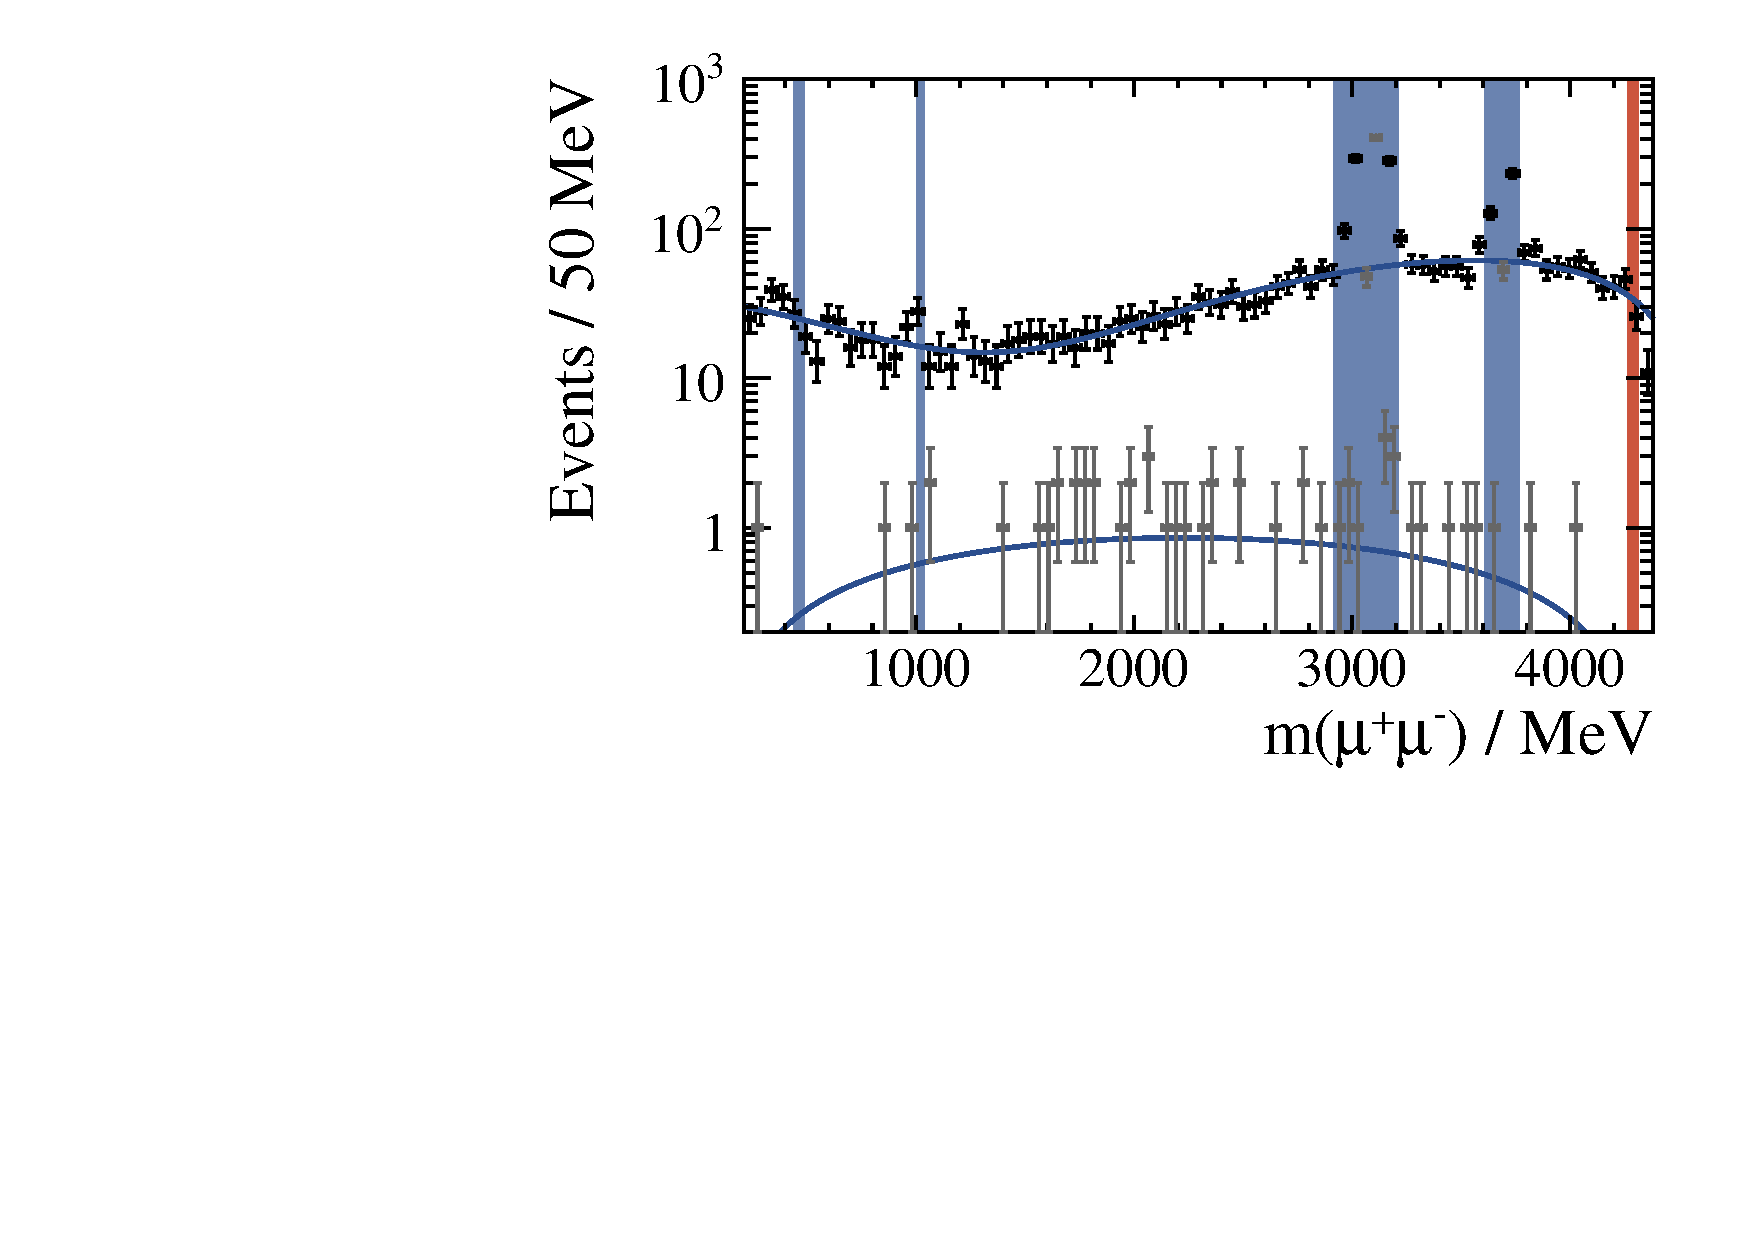
\includegraphics[width=0.48\textwidth]{mxpdf}
    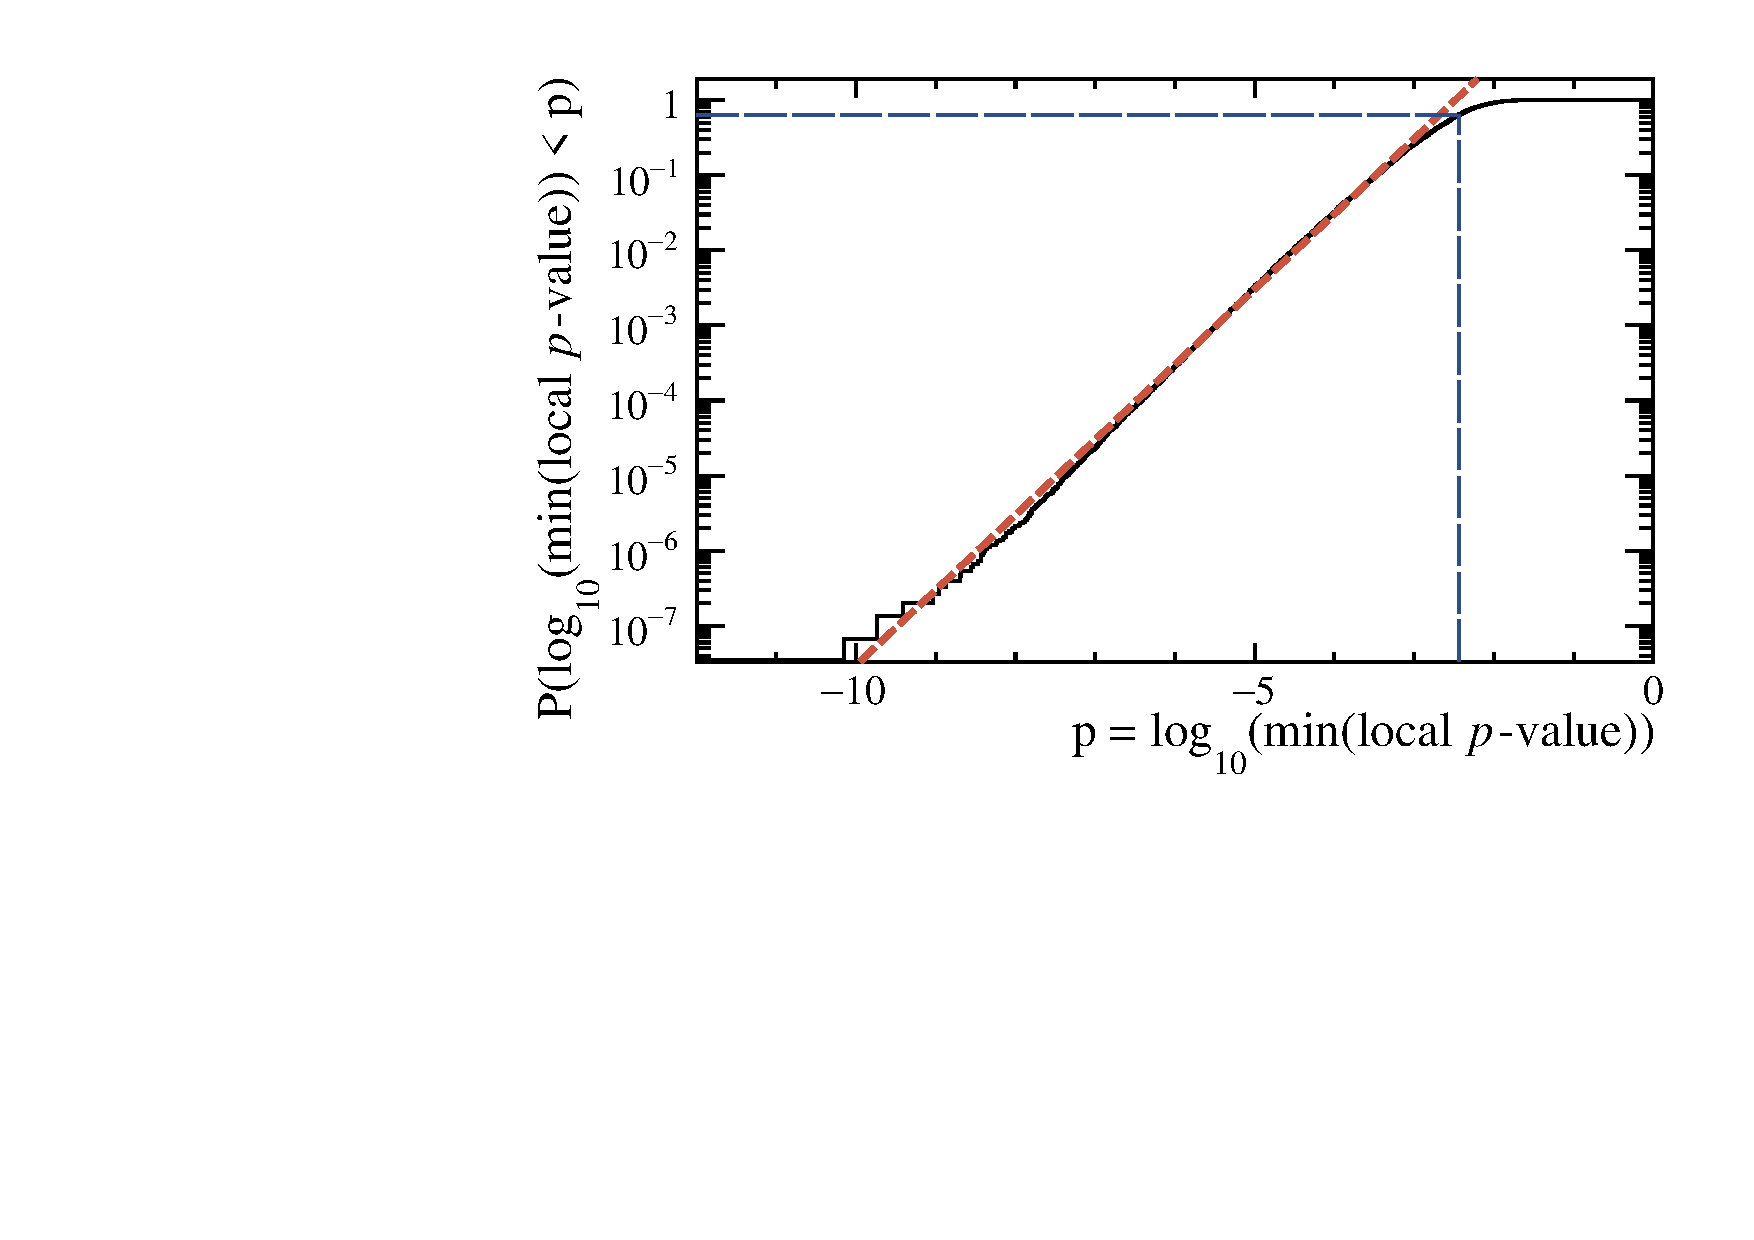
\includegraphics[width=0.48\textwidth]{pvalConversion}
    \caption[]
    {
      %Invariant mass of dimuon pairs from the selection
    }
    \label{fig:db:mmumu}
  \end{center}
\end{figure}


%Scanning values of \mass{t} in the ranges:
%
%The minimum local $p$-value observed in data is $xxx$  at $\mass{\mumu}xxx\mev$,
%which corresponds to a global $p$-value of $xxx$; corresponding to a shift in significance of
%$xxx\stdev$ to $xxx\stdev$.



%Reference~\cite{Bezrukov:2009yw} considers inflatons with masses in the range
%$1<\mass{\db}<1000\mev$ with lifetimes in the




%From this \PDF ten million toy datasets are generated,
%Ten million are required to be sensitive to

%Using the unblinded
%A fourth order Chebychev polynomial is fit to the unblinded \mass{\mumu} distribution,
%these data
%and
%from this, ten million toy datasets are generated.
%A least ten million are needed in order to be able to probe to $p$-values of $5\stdev$.

%The resulting \qsq distribution is shown in \Fig{fig:res:q2} along with a fit to

%\section{Blinded distributions}
%\label{sec:results}

%Figure~\ref{fig:res:mbvtau}, shows the \db candidate lifetime against \Bd
%mass, it also shows the effect the uBDT cut has on the combinatorial background.
%The lifetime of the \db candidate is also shown as a function of the \db mass, inside and outside
%the \Bd signal region in Fig~\ref{fig:res:mxvtau}.

%%\begin{figure}
  %%\begin{center}
    %%\subfloat[\label{fig:res:mbvtau:all}]{\includegraphics[width=0.48\textwidth]{mb_v_tau}}
    %%\subfloat[\label{fig:res:mbvtau:bdt}]{\includegraphics[width=0.48\textwidth]{mb_v_tau_bdt}}
    %%\caption{\small
      %%Distributions of $\tau(\mumu)$ against $m(\Kstarz\mumu)$ for
      %%candidates from data
      %%\protect\subref{fig:res:mbvtau:all} with no cut, and
      %%\protect\subref{fig:res:mbvtau:bdt} with a cut on the uBDT classifier.
      %%The signal region has been blinded.
    %%}
    %%\label{fig:res:mbvtau}
  %%\end{center}
%%\end{figure}
%%
%%\begin{figure}
  %%\begin{center}
    %%\subfloat[\label{fig:res:mxvtau:all}]{\includegraphics[width=0.48\textwidth]{mx_v_tau}}
    %%\subfloat[\label{fig:res:mxvtau:sig}]{\includegraphics[width=0.48\textwidth]{mx_v_tau_sig}}\\
    %%\subfloat[\label{fig:res:mxvtau:bdtall}]{\includegraphics[width=0.48\textwidth]{mx_v_tau_bdt}}
    %%\subfloat[\label{fig:res:mxvtau:bdtsig}]{\includegraphics[width=0.48\textwidth]{mx_v_tau_sig}}
    %%\caption{\small
      %%Distributions of $\tau(\mumu)$ against $m(\mumu)$ for \db candidates from data in the
      %%\protect\subref{fig:res:mxvtau:all} upper mass sideband, and
      %%\protect\subref{fig:res:mxvtau:sig} signal region (without the uBDT applied).
      %%The Figs.~\protect\subref{fig:res:mxvtau:bdtall} and \protect\subref{fig:res:mxvtau:bdtsig} show the
      %%same, but with uBDT cut applied (blank plots emphasize the analysis is blind).
      %%%\emph{Blank plots will be filled in after unblinding.}
    %%}
    %%\label{fig:res:mxvtau}
  %%\end{center}
%%\end{figure}




\subsection{Systematic uncertainties}
Systematic uncertainties must be assessed in order to set limits.
Sources of systematic uncertainties are from:
the ratio of efficiencies $\varepsilon(\btokstrdb)/\varepsilon(\btokstrmumu)$;
the definition of prompt and displaced regions;
and the uncertainty on the \sm \btokstrmumu normalization yield.

The efficiency ratio $\varepsilon(\btokstrdb)/\varepsilon(\btokstrmumu)$ is approximately one, by
construction, for each mass at zero lifetime.
For larger lifetimes, the efficiency can be checked using data consistent with the decay
\decay{\Bd}{\jpsi\KS}.
It should be noted that in the displaced region a large uncertainty on the efficiency ratio will
translate to a small uncertainty in the limits, because of the low statistics in that region.

%Systematic checks addressed using \Bd mass peak in low \qsq region CONF
%only relative efficiensy between signal and sm is reqiored, should be about 1 by construction, as
%seen in..

%For large decay times, must validate large-lifetime effs, using b to jpsi ks, but, due to low
%background in displaced region, even a 20\% relative uncertainty will only increase limits by \bout
%2\%.

Studies undertaken in \Ref{Williams:2015xfa} show that the defining the boundary that separates
the prompt and displaced regions to be $3\sigma_\tau$ is nearly optimal for any value of
\lifetime{\db}.
Only if $\lifetime{\db}\simeq3\sigma_\tau$, then there may be some effect on the limits.
The total effect of this must be demonstrated.

An important consideration is the spin of the \db.
Since the spin of the \db is unknown, there are a range of possible angular distributions that may
arise, each having a different detection efficiency.
This can be studied using the angular acceptance models used in the \btokstrmumu angular
analysis~\cite{LHCb-CONF-2015-002}.
%The model with which the simulated samples were produced assumes that the \db is a scalar, a vector
%there may be devaiation
%
%dominant contribution for $\tau\sim0$ comes from unknown spin of \db, angular distributions, can
%use angular acceptance model in sm.

It has been noted that this analysis relies on the assumption that the background is smoothly
varying, and can be approximated as being locally linear.
This assumption clearly introduces an uncertainty, but this is already accounted for in the method
by the addition of the Gaussian, $\mathcal{G}(y, x, \sigma_y)$, in the likelihood shown in
\Eq{eq:db:like2}.
There is no need to add a systematic uncertainty for the chosen value of $\sigma_y$, because it is,
itself, and uncertainty and a maximal one.

%Sources of systematic uncertainties that are considered come from the ratio of efficiencies
%ratio of eff
%counting of signal events in prompt and displaced









